\documentclass{article}
\usepackage{graphicx}
\usepackage{subfigure}
%\usepackage{subfig}
\begin{document}
\section{Tag Frequency Diagrams}
\subsection{Experiment Setup}
\paragraph{The Input Blocks of Tags}
In this experiment, the length of a input block, D, to CETD is 16 bits.The hexadecimal domain of D block is [0x0000, 0xFFFF].  The tag length is set to 8 bits, so the input block D is splited into two sub-blocks D$_a$ and D$_b$. Each sub-block has a length of 8 bits.

Our experiment simulate the replay attack. Using each distinct value in the domain of D as input to CETD, we generated 1000 tags. For the input of nonce for each tag, the following two principles is met:
\begin{itemize}
	\item The counter is distinct
	\item The random number is randomly generated by PRF
\end{itemize}
Hence the block cipher we use in nonce generation is AES, each nonce in the 1000 times tag generation is randomly generated. 
We want to examine the distribution of distinct tag values for each distinct D block. 





\subsection{The Results}
\begin{figure}[htbp]
 \centering
 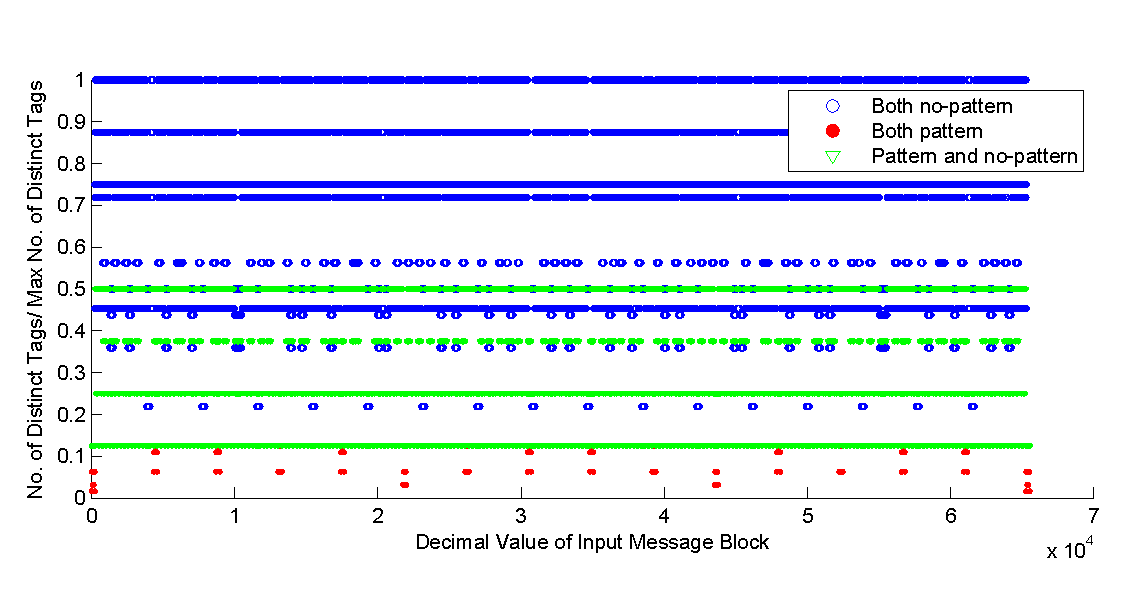
\includegraphics[scale=0.6]{./frequency/pattern_no_mix_frequency_new.pdf}
 \caption{The tag value frequency diagram for all D blocks. Y axis expresses the frequency of tag values of a D value divided by the maximum frequecy}
 \label{frequency_plot }
\end{figure} 
\paragraph{The Frequency Diagram of D Values}
The tag frequency diagram of all D values is expressed in Figure 1. From the figure we can see that the frequency of tag varies to different levels. Tag frequency of D values that none of its sub-block is expressed with blue circle; green triangle represent the tag frequency of D values which has a pattern sub-block; red "*" represents the tag frequency of D values whose both sub-blocks are formed by pattern. 
Figure 2. enlarge a part of Figure 1 to help clarify the tag frequency of each D block. 
\begin{figure}[htbp]
 \centering
 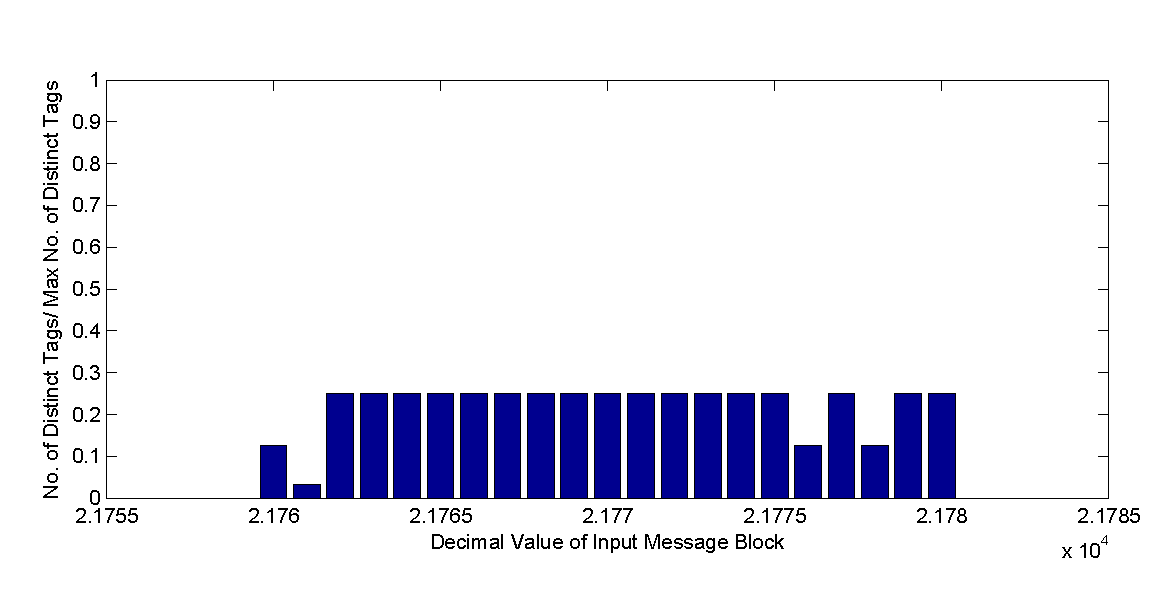
\includegraphics[scale=0.4]{./frequency/portion_bar.pdf}
 \caption{The tag value frequency diagram for a part of D blocks}
 \label{frequency_hist }
\end{figure} 
As analyzed before, the tag has more probability to collide under replay attack if each sub-block of D is formed by a pattern. From Fig 1 we can see that red spots have lowest value of frequency. When one of the sub-block is formed without pattern, the frequency values represent by green triangle reach a high value.

\paragraph{The no-pattern D values that result to low tag frequency}
 
\end{document}